\thislesson{23 Gennaio 2017}{Biliardi ellittici e Supercazzole immaginarie}

\section{Biliardi ellittici}
\newthought{Introduciamo un altro modo} in cui si ottengono le curve
ellittiche dalle ellissi \notamargine{Abbiamo infatti già visto che si
  possono ottenere come integrali della lunghezza d'arco di un'ellisse}.

Prendiamo un'ellisse di equazione $ax^2 + by^2 = 1$ e supponiamo di
giocare a biliardo sull'ellisse: facendo partire la pallina da un punto
la lanciamo contro il bordo dell'ellisse su cui rimbalza secondo la nota
legge della riflessione \notamargine{Ovvero rispetto alla tangente
  all'ellisse nel punto rimbalza via con lo stesso angolo, come indicato
  in figura}

\begin{center}
  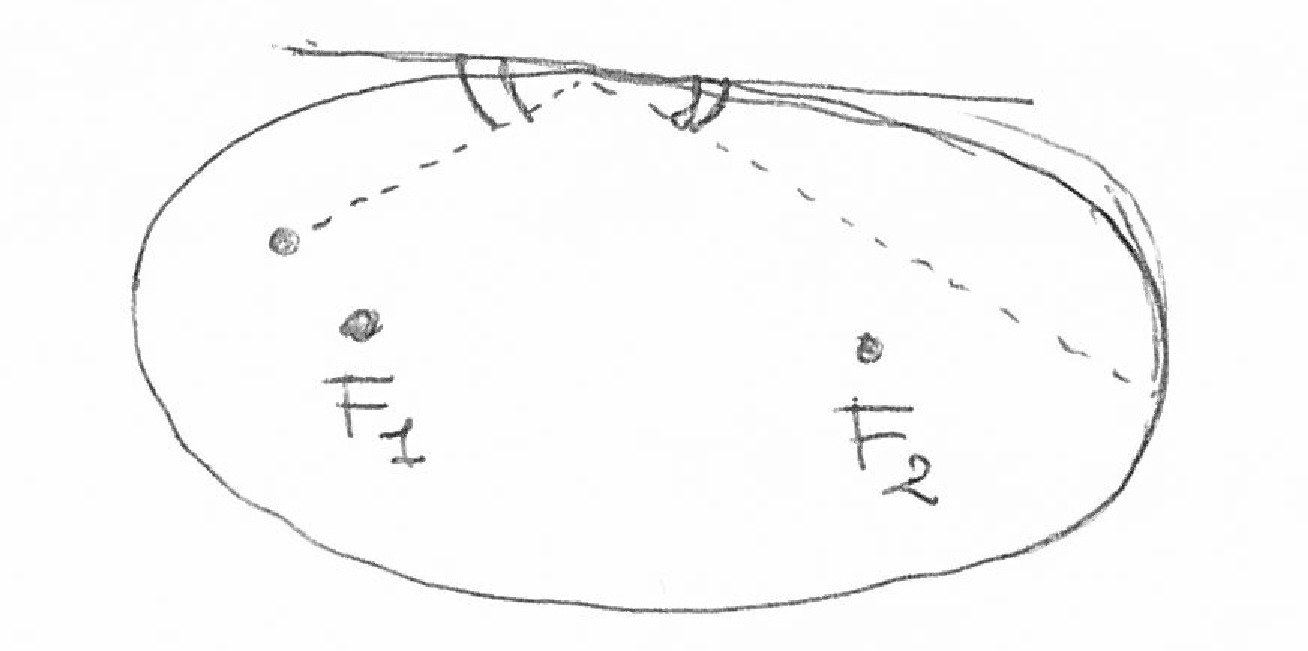
\includegraphics[width=8cm]{lezione-170123-fig1}
\end{center}

Una cosa che è nota da tempo è che le rette che compongono la
traiettoria sono tutte tangenti ad un'altra ellisse ``caustica'' che ha
gli stessi fuochi della prima: abbiamo quindi una famiglia ad un
parametro di ellissi che descrive tutte le possibili traiettorie.

\newthought{Vediamo allora che succede} quando prendiamo un punto $P$
sul bordo dell'ellisse ed una retta $l$ con $P \in l$ e tangente alla
caustica:

Possiamo definire un'applicazione $\phi$ dalle coppie punto-retta in sè
che è la funzione di ``evoluzione'' della traiettoria sul biliardo,
ovvero manda la coppia $(P, l)$ in $(P', l')$ con $P'$ l'altro punto di
intersezione della retta $l$ con l'ellisse e $l'$ la retta passante per
$P'$ che segue la legge della riflessione con $l$.

\notamargine{
  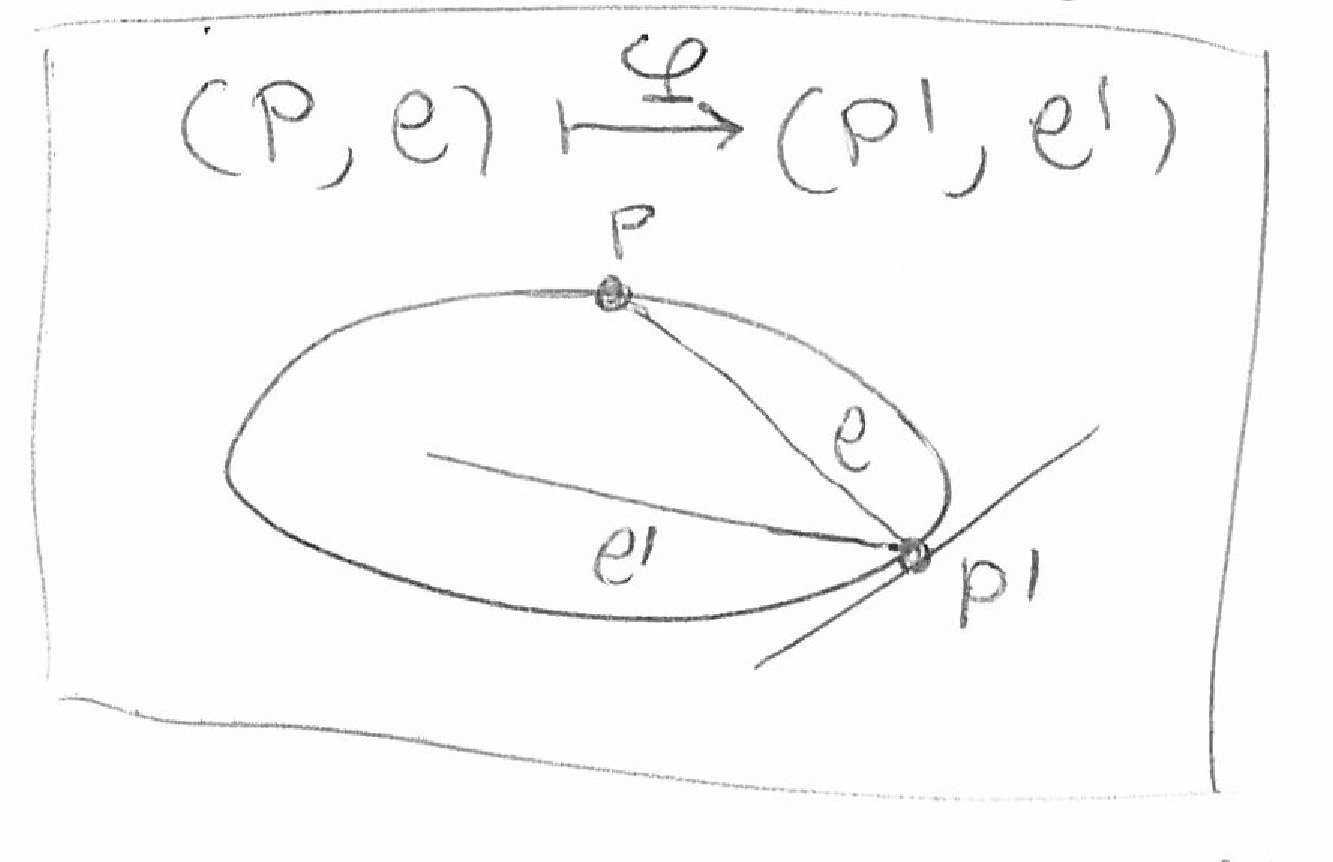
\includegraphics[width=4cm]{lezione-170123-fig2}
}

\newthought{È noto} che le tangenti in $\bbP^2$ ad una conica sono
parametrizzate da un'altra conica: la conica duale.
\notamargine{Tutto ciò non è difficile da verificare: se la conica $\cC$
  ha equazione $f = ax^2 + by^2 + cz^2$ e $(x_0, y_0, z_0) = P \in \cC$
  allora $(\nabla f)_P = (2ax_0, 2by_0, 2cz_0)$ e, ricordando che tutti
  i punti/vettori considerati sono in $\bbP^2$ si ha che dare la retta
  tangente in $P$ è uguale a fornire il vettore $(\nabla f)_P$. D'altra
  parte si riesce ovviamente a recuperare il punto $P$ dato $(\nabla
  f)_P$ a cui è tangente (basta vedere la formula scritta sopra in
  coordinate, visto che i coefficienti della conica sono noti)}
Allora il luogo di punti su cui la $\phi$ agisce è una sottovarietà
(algebrica) di $C_1 \times \hat{C_2}$, con $C_1 = \text{punti della
  conica}$ e $\hat{C_2} = \text{conica duale delle rette tangenti}$.

Il luogo di punti è dato dalle coppie $(P, l) \in C_1 \times \hat{C_2}$
tali che $P \in l$ (che è una condizione chiusa, ovvero dà luogo ad una
sottovarietà algebrica). Questa è anche una superficie di Riemann.

Scrivendo l'equazione si ottiene una curva ellittica e l'operazione
$\phi$ si rivela essere una traslazione sulla cubica detta ``gioco di
Poncelèt''.

Il gioco ``finisce'' se e solo se la traslazione $\phi(x) = x + \tau$ ha
un punto di ordine finito, ovvero $\exists n$
$\phi^n (x) = x + n\tau = x$ se e solo se $n\tau \in L$, il
reticolo. Ovvero si avrebbe $\phi^n(x) = x$ per ogni punto. Allora se il
gioco finisce per una traiettoria finisce per tutte le altre, cosa che
non è per nulla banale.

\notamargine{Come curiosità, se il gioco non finisce, le traiettorie del
  biliardo sono dense nello spazio tra le due ellissi}

\section{Funzioni Modulari}

\notamargine{Il nome ``modulari'' è riferito ai moduli, parametri che
  comparivano negli integrali ellittici. Oggi ci si riferisce a moduli
  per indicare uno spazio di parametri per una famiglia di curve
  algebriche.

  Esempio ``stupido'': $y - a x^2 = 0$ al variare di $a \in \bbC$ sono
  una famiglia di parabole (o per $a=0$ una retta). In questo caso lo
  spazio dei parametri è $\bbC$ (nel quale $a$ può variare)}

\begin{osservazione}
  Ricordiamo che conosciamo già un parametro delle cubiche:
  $j$. Infatti, se la cubica viene da un toro allora è della forma
  $y^2 = 4 x^3 - g_2 x - g_3$ e sappiamo che
  $j = 1728 \frac{g_2^3}{g_2^3 - 27 g_3^2}$ è un'invariante per
  trasformazioni proiettive delle cubiche.
\end{osservazione}

Siamo allora autorizzati a riscalare il reticolo $L$ pur restando nella
stessa classe di isomorfismo delle cubiche. Possiamo quindi supporre che
$L = \bbZ \tau + \bbZ 1$ con $\tau \in \cH = \{ z \in \bbC | \Img \tau >
0 \}$. In questo modo $g_2 = 60 \sum_{\omega \in L^*} \omega^{-4}$ e
$g_3 = 140 \sum_{\omega \in L^*} \omega^{-6}$ diventano funzioni
olomorfe di $\tau$ come parametro nel semipiano superiore e quindi pure
$j$ è una funzione di $\tau$

\begin{osservazione} \label{170123-j_suriettiva}
  Se vedessimo che $j$ assume tutti i valori in $\bbC$ ciò dimostrerebbe
  che tutte le cubiche provengono da un toro, poiché sappiamo già che
  due cubiche sono affinemente equivalenti se e solo se hanno lo stesso $j$.
\end{osservazione}

\begin{divagazione}
  Si può dimostrare che se $\tau$ è immaginario quadratico su $\bbQ$ allora
  $j(\tau)$ è un numero algebrico. Di seguito diamo una supercazzola della dimostrazione
  \notamargine{Immaginario quadratico vuol dire che soddisfa
    un'equazione di secondo grado a coefficienti in $\bbQ$, ovvero $x$ è
    tale che $\exists b, c \in \bbQ$ con $x^2 + bx + c = 0$ e che è un
    numero immaginario puro}

  Quando $\tau$ è un immaginario quadratico il reticolo ha infatti degli
  endomorfismi non banali. Se $j$ fosse trascendente, visto che gli
  endomorfismi sono funzioni razionali delle coordinate e avremmo
  $\bbQ(j, \text{funz.raz.})$ come campo finitamente generato su $\bbQ$,
  che ha grado di trascendenza uno.

  Allora si può ``specializzare'' $j$, visto che il campo è isomorfo ad
  una cosa con una variabile.

  \notamargine{Qui intendiamo ad esempio che $\bbQ(j, \sqrt{j + 2})
    \cong \bbQ(t, \sqrt{t + 2})$ con $t$ come variabile e quindi $\cong
    \bbQ(t_0, \sqrt{t_0 + 2})$ con $t_0$ trascendente.}

  Specializzandolo ad ogni altro numero trascendente ottengo un campo
  isomorfo e quindi tutte le curve ellittiche avrebbero degli
  automorfismi non banali (poiché hanno uguali campi) e ciò è
  impossibile poiché le cubiche con automorfismi sono in numero
  numerabile.
\end{divagazione}

Il reticolo $L$ può avere altre basi, date dall'applicazione di matrici
$\kM_{2 \times 2} (\bbZ)$ invertibili. Possiamo scegliere l'ordine dei
due elementi della base in modo da avere soltanto le matrici con
determinante uno.

Diciamo che due reticoli $\bbZ + \bbZ \tau = \bbZ + \bbZ \tau'$ sono
equivalenti se $\exists g \in \SL_2 \bbZ$
$\tc g\tau = \tau' = \frac{a \tau + b}{c \tau + d}$

Allora i tori complessi modulo isomorfismo sono in biggezione con $\cH$
modulo $\SL_2 \bbZ$ (in realtà l'azione si quozienta per $\{\pm 1\}$,
quindi l'azione è di $\bbP\SL_2 \bbZ$).

\section{Costruzione di un dominio fondamentale}

Vogliamo costruire un dominio fondamentale per lo spazio dei reticoli,
ovvero su cui agiranno le funzioni modulari.
\notamargine{Per dominio fondamentale intendiamo uno spazio in cui è
  presente esattamente un rappresentante per ogni reticolo. Nel nostro
  caso portiamo ogni reticolo nella forma $L = \bbZ + \bbZ \tau$}

Descriviamo innanzitutto la forma del dominio fondamentale:
$ F = \cH \cap \{ \Re z \in [ -\frac{1}{2}, \frac{1}{2} ) \} $
tolto l'insieme $\{ \abs{z} < 1 \} \cup \{ \abs{z} = 1 \mid \Re z > 0 \}$

e definiamo le due applicazioni
$$ S = \lbr{\begin{array}{cc} 0 & 1 \\ -1 & 0 \\ \end{array}} $$
$$ T = \lbr{\begin{array}{cc} 1 & 1 \\ 0 & 1 \\ \end{array}} $$
tra cui si hanno le relazioni $S^2 = (TS)^3 = \Id$

\begin{center}
  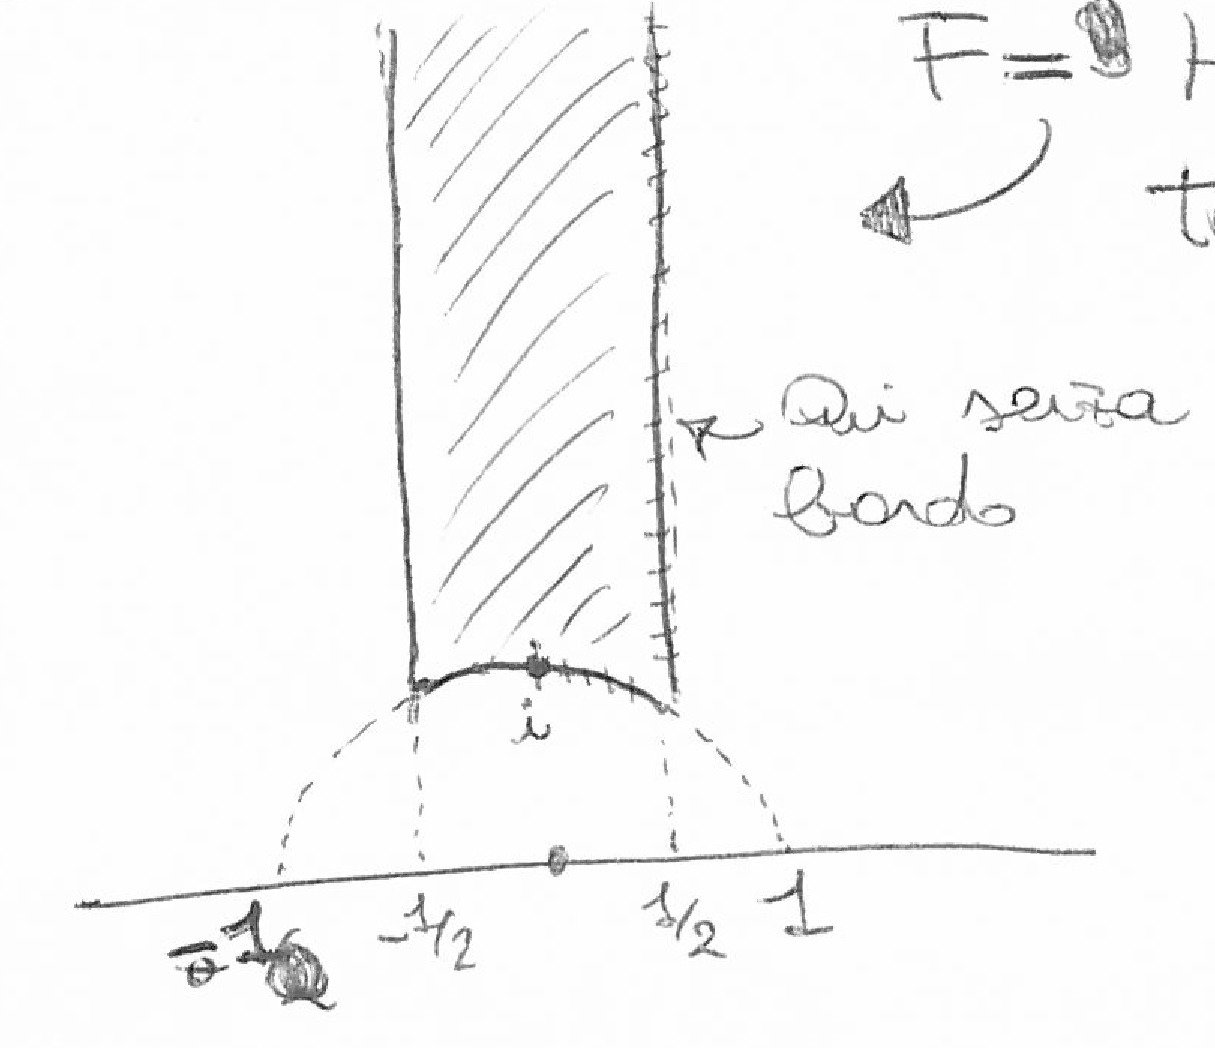
\includegraphics[width=8cm]{lezione-170123-fig3}
\end{center}

\begin{osservazione}
  Sarà parecchio importante sapere che se
  $g = \lbr{\begin{array}{cc} a & b \\ c & d \\ \end{array}} \in
  \SL_2(\bbZ)$, allora si ha $\Im (gz) = \frac{\Im z}{\abs{cz + d}^2}$.
\end{osservazione}

\begin{lemma}
  $\SL_2 \bbZ$ è un sottogruppo discreto come sottoinsieme di $\SL_2 \bbR$
  ed agisce in modo propriamente discontinuo su $\cH$
\end{lemma}
\begin{proof}
  Sia $K \subseteq \cH$ un compatto: vogliamo mostrare che allora
  $gK \cap K \neq \emptyset$ per al più un numero finito di $g \in G$.

  Allora sia $z_0 \in K$ tale che $g z_0 \in K$. Sappiamo però che per
  un qualunque compatto in $\cH$ $\exists \rho, \rho'$ che dipendono
  solo dal compatto tali che $\rho' > \Im z > \rho > 0$ per un qualunque
  $z \in K$. Se anche $g z_0 \in K$ ne segue allora che $\abs{cz_0 + d}$
  è limitato uniformemente in $z_0$ $\implies$
  $\Im (cz_0 + d) = c \Im z_0$ $\implies$ $c$ è limitato ed anche $d$ è
  limitato (e la limitazione dipende solo da $K$)

  $\frac{a z_0 + b}{c z_0 + d} \in K$. Allora, visto che le possibili
  coppie $(c, d)$ sono finite, si ha
  $a z_0 + b \in \cup_{(c, d)} (cK + d)K$ che è compatto e quindi si
  conclude come sopra (utilizzando $\rho$ e $\rho'$)
\end{proof}

Anche se l'azione è propriamente discontinua il quoziente non è comunque
rivestito perché ci sono dei punti fissi: ad esempio $Si = i$ e $ST
\zeta_3 = \zeta_3$. Ma sono gli unici due punti che danno fastidio.

\notamargine{Incollando i bordi del dominio fondamentale si può vedere
  che topologicamente lo spazio delle curve ellittiche è omeomorfo a
  $\bbC$, anche se ovviamente non può esserne biolomorfo né rivestito
  per le conseguenze del teorema di classificazione di Riemann}

Nella prossima lezione vedremo il teorema che ci mostra che $F$ come
descritto è effettivamente un dominio fondamentale e, come curiosità:
\begin{teorema}
  $G = \SL_2 \bbZ$ è generato da $S$ e da $T$. Inoltre è esattamente il
  gruppo libero su due elementi ($S$ e $T$) con le relazioni
  $S^2 = (TS)^3 = \Id$
\end{teorema}

\thislesson{31 Gennaio 2017}{Azione di $SL_2 \left( \bbZ \right)$ su $\cH$ e Funzioni Modulari}

\section{Azione di $SL_2 \left( \bbZ \right)$ su $\cH$}

Siano $F=\left\{z \in \cH | -\frac{1}{2} \leq \Re(z) \leq 0
\wedge |z| \geq 1 \right\} \cup
\left\{z \in \cH | 0 < \Re(z) < \frac{1}{2} \wedge |z| > 1 \right\}$,
$G=SL_2 \left( \bbZ \right)/\{\pm Id\}$,   $\rho=\frac{-1+i\sqrt{3}}{2}$,
$S=\left( \begin{array}{cc} 0 & 1 \\ -1 & 0 \end{array} \right) \in G$,
$T=\left( \begin{array}{cc} 1 & 1 \\ 0 & 1 \end{array} \right) \in G$,
$G' = \langle S, T \rangle$.

\begin{teorema}
\begin{itemize}
\item[P0] $\forall z \in \cH \quad \exists g \in G$ tale che $gz \in F$
\item[P1] se $z,gz \in \bar{F}$ con $g \neq \Id$, allora $z \in \partial F$.
  Più precisamente si hanno i tre casi (anche se non disgiunti):
  \begin{enumerate}
  \item[C1] $\Re z = \pm \frac{1}{2}$ e $z' = z \mp 1$
  \item[C2] $|z| = 1$ e $z' = - \frac{1}{z}$
  \item[C3] $z = z' = \rho$ oppure $z = z' = \rho + 1$
  \end{enumerate}
\item[P2] se $z \in F$ e $z=gz$,
  allora $z=i$ (nel qual caso $g \in \left\langle S \right\rangle$) oppure si ha che
  $z= \rho$ (nel qual caso $g \in \left\langle ST \right\rangle$)
\end{itemize}
\end{teorema}

\begin{proof}
  \squared{P0}
Sia $G'=\left\langle S,T \right\rangle$. Sia $z \in \cH$ e cerchiamo $z' \in G'z$ con $\Im(z')$ massima possibile. Tale elemento esiste, infatti se
$\sigma = \left( \begin{array}{cc} a & b \\ c & d \end{array} \right) \in G'$, allora $\Im(\sigma z) = \frac{\Im(z)}{|cz+d|^2}$ ed essendo
$c,d \in \bbZ$, $|cz+d|^2 \geq (\Im(z))^2$ (per $c \neq 0$, se no fa $d^2 \ge 1$) per cui $\Im(\sigma z)$ è limitato dall'alto e il sup viene raggiunto perché
ci sono solo un numero finito di $c,d \in \bbZ$ per cui $|cz+d|^2 \leq 1$. (Infatti siccome lo cerco massimo voglio denominatore più piccolo di uno,
altrimenti già $z$ andava bene)

\notamargine{Per vedere che ve ne sono un numero finito scriviamo $|cz+d|^2 = c^2 (\Im z)^2 + (c \Re z + d)^2 \le 1$.
  Allora ciascun termine è minore di $1$, quindi ci sono un numero finito di $c$, e da questo si ricava che vi sono un numero finito di $d$.}

Possiamo quindi supporre che $z=z'$ e, a meno di comporre con qualche potenza
di $T$ (che è una traslazione), supponiamo anche che $-\frac{1}{2} \leq \Re(z) < \frac{1}{2}$.

Verifichiamo quindi che $|z| \geq 1$ (se poi fosse $|z|=1$ e
$z \in \bar{F} \setminus F$ basta applicarci $S$).
$\frac{\Im(z)}{|z|^2} = \Im(Sz) \leq \Im(z)$ per la massimalità di $\Im(z)$.
Quindi $|z| \geq 1$.
\vskip 0.5cm

\squared{P1}
Siano ora $g \in G$, $z'=gz$ e supponiamo che $z,z' \in \bar{F}$ e (wlog)
che $\Im(z) \leq \Im(z')$.
$$
z'= gz \cdot 1 = \frac{az+b}{cz+d} \frac{c \bar{z} +d}{c \bar{z} +d} =
\frac{ac|z|^2 + bd + bc \bar{z} + adz}{|cz+d|^2} \stackrel{det=1}{=}
\frac{ac|z|^2 + bd + bc \bar{z} + (bc+1)z}{|cz+d|^2} =
$$
$$
\frac{ac|z|^2 + bd + bc (\bar{z} + z) + z}{|cz+d|^2} =
\frac{ac|z|^2 + bd + (2bc+1) \Re(z)}{|cz+d|^2} + i \frac{\Im(z)}{|cz+d|^2}
$$
Ora, usando che $z,z' \in \bar{F}$, per cui $|z|,|z'| \geq 1$ e
$|\Re(z)|, |\Re(z')| \leq \frac{1}{2}$, si ottiene che, se $c \neq 0$,
$\Im(z') = \frac{\Im(z)}{|cz+d|^2} \leq \frac{\Im(z)}{c^2 \Im(z)^2}
= \frac{1}{c^2 \Im(z)} \leq \frac{2}{c^2 \sqrt{3}}$ $\implies c^2 \le \frac{2}{\sqrt{3}\Im z'} \le \frac{4}{3}$
quindi $|c| \leq 1$.

\begin{itemize}
\item Se $c=0$, allora (visto che $ad - bc = 1$) deve essere $z' = z \pm b$, per cui si può avere $z'=z$ e $g=Id$; oppure
  $|\Re(z')| = \frac{1}{2}$ e $|\Re(z)| = -\frac{1}{2}$; o viceversa.
  \notamargine{Nel caso $c=0$ stando $z, z' \in F$ si ha $|\Re z - \Re z'| \le 1$}
  Negli ultimi due casi si ha $z,z' \in \partial F$ e $g=T$ e vale C1.

\item Se invece $c=1$ (il caso $c=-1$ è uguale perché
  $G=SL_2 \left( \bbZ \right)/\{\pm Id\}$),
  $\Im(z') \leq \frac{1}{\Im(z)} \stackrel{z' \in F}{\Rightarrow} \Im(z) \leq \frac{2}{\sqrt{3}}$.
  Allora $\Im(z') \leq \frac{2}{\sqrt{3}|z+d|^2} \Rightarrow
  |z+d|^2 \leq \frac{4}{3} \Rightarrow |z|^2+d^2+2d \Re(z) \leq \frac{4}{3}$.
  Quindi (poiché $\Re z \ge -\frac{1}{2}$) $d=0$ o $d=\pm 1$.

  Se $d=0$, $\Im(z') = \frac{\Im(z)}{|z|^2} \leq \Im(z)$, quindi $|z|=1$ (Perché avevamo precedentemente assunto che $\Im(z) \le \Im(z')$).
  Considerando il determinante si ottiene $b = -1$ e quindi $z' = \frac{az - 1}{z} = a - \frac{1}{z} = a - \bar{z}$. Siccome $z$ è sulla circonferenza unitaria anche $- \bar{z}$ lo è; visto che sia $z'$ che $z$ devono stare in $F$, deve essere $a = 0, \pm 1$.
  \begin{itemize}
  \item $a = 0$. Allora siamo nel caso C2
  \item $a = \pm 1$ allora $z = z' \in \{\rho, \rho + 1\}$ e siamo nel caso C3
  \end{itemize}

  Se $d=\pm 1$, similmente $\Im(z') = \frac{\Im(z)}{|z \pm 1|^2}$. Usando che $|z \pm 1| \ge 1$ (Fare disegno e cercare minimo modulo di $F + 1$)
  si ottiene $|z \pm 1|=1$, da cui, di nuovo, $z=\rho, z'=\rho + 1$ o viceversa e siamo nel caso C1.
\end{itemize}

\bigskip
\squared{P2} Utilizzando il punto P1 distinguiamo i tre casi:
\begin{itemize}
\item Il caso C1 non si realizza perché avevamo $z' \neq z$
\item Il caso C2 ci da $z^2 = -1 \implies z = i$ e, per quanto visto sopra, si ha $g = S$
\item Il caso C3 ci da solo $z = z' = \rho$ perché $\rho + 1 \notin F$ e si ottiene $g = \left(\begin{array}{cc} -1 & -1 \\ 1 & 0 \\ \end{array} \right) = (ST)^2$, quindi (visto che $(ST)^3 = \Id$) lo stabilizzatore è il sottogruppo $\langle ST \rangle$
\end{itemize}
\end{proof}

\begin{corollario}
F è un dominio fondamentale.

$Stab(i)=\left\langle S \right\rangle$,
$Stab(\rho)=\left\langle ST \right\rangle$ e $Stab(z)=\emptyset$ se
$z \notin \{i, \rho \}$.
\end{corollario}

\begin{teorema}
G è generato da S e T
\end{teorema}

\notamargine{In realtà si potrebbe dimostrare anche che G è il gruppo libero
generato da $S$ e $T$ modulo le relazioni $S^2=Id$ e $(TS)^3=Id$}

\begin{proof}
Vediamo ora che $G'=G$:

Sia $z=2i$ e sia $g \in G$. Per quanto visto sopra, $\exists \sigma \in G'$
tale che $\sigma g(z) \in \bar{F}$. Allora, dato che $z \notin \partial F$,
$\sigma g(z)=z$.
Poiché gli unici stabilizzatori non banali sono quelli
previsti dal corollario, ne deduciamo che $\sigma g = Id$ e quindi $G=G'$.
\end{proof}

\begin{osservazione}
  Al quoziente $\cH/G \simeq F$ si può dare una struttura di superficie di Riemann
  (che non è quella data dall'immersione per via dei due stabilizzatori non banali),
  identificando le rette $\Re(z)=\pm \frac{1}{2}$ e i due archi di circonferenza
  (quelli passanti per $i$) sul bordo di $F$. Il quoziente è omeomorfo a $\bbC$.
  Possiamo quindi indurre una struttura di superficie di Riemann con l'omemomorfismo trovato.
\end{osservazione}

\section{Forme quadratiche binarie intere}
Una forma quadratica binaria intera è un'espressione del tipo:
$$ ax^2+bxy+cy^2 \qquad a,b,c,d \in \bbZ $$
Si vogliono classificare a meno di equivalenza lineare con elementi di
$SL_2 \left( \bbZ \right)$.

\begin{osservazione}
Il discriminante $\Delta =b^2-4ac$ è invariante per trasformazioni lineari
invertibili. Inoltre, fissato $\Delta$, il numero di classi di equivalenza con
quel discriminante è FINITO (questo però è difficile).
Quando $\Delta < 0$, è utile considerare $\xi \in \cH$ che risolve
$a \xi^2 + b \xi + c =0$. Per quanto abbiamo visto, $\exists \sigma \in G$
tale che $\sigma \xi \in F$. Tramite $\sigma$ si ottiene la forma ridotta secondo
Gauss.
\end{osservazione}

\section{Funzioni Modulari}
\begin{definizione}
Una funzione $f$ meromorfa su $\cH$ di dice debolmente modulare di peso $2k$ (per $k \in \mathbb{N}$), se $\forall
\left( \begin{array}{cc} a & b \\ c & d \end{array} \right) \in
SL_2 \left( \bbZ \right)$ si ha:
$$ f\left( \frac{az+b}{cz+d} \right) = (cz+d)^{2k} f(z)
\qquad \forall z \in \bbC$$
\end{definizione}

\begin{osservazione}
$\displaystyle{gz=\frac{az+b}{cz+d} \stackrel{\det = 1}{\Rightarrow}
\frac{d(gz)}{dz}=\frac{1}{(cz+d)^2}}$. Quindi la condizione della definizione di
funzione debolmente modulare può essere scritta come $f(gz)(d(gz))^k=f(z)(dz)^k$.
Sono k-forme differenziali (secondo noi però sono tensori $(0, k)$ simmetrici).
\end{osservazione}

\begin{osservazione}
Dalla definizione segue immediatamente che $f(z+1)=f(z)$, cioè che una
funzione debolmente modulare è periodica di periodo $1$. Definendo $q(z) = e^{2 \pi i z}$
si ha che $q$ manda $\cH$ in $D^*$ (e in particolare $\cH / \bbZ \simeq D^*$), quindi
$\widetilde{f} = f \circ q^{-1}$ è meromorfa in $D^*$ e
$\displaystyle{\sum^{+\infty}_{n=-\infty}{a_n q^n}}$ è la sua serie di Laurent.
Quindi $f$ si può scrivere in ``serie di Fourier'' in $q=e^{2 \pi i z}$, cioè
$\displaystyle{f(z)=\widetilde{f}(q)=\sum^{+\infty}_{n=-\infty}{a_n q^n}}$.
\end{osservazione}
\notamargine{Non capiamo bene come si possa dedurre la sviluppabilità in serie di Laurent
  (i poli potrebbero accumularsi in $0$). Si può invece ben fare se $f$ è una funzione modulare,
  definita poco più sotto.}

\begin{definizione}
Nelle notazioni di sopra, se $\widetilde{f}$ è meromorfa anche in $D$, cioè
se gli $a_n$ con indice $n<0$ non nulli sono in numero finito, la $f$
è "meromorfa all'$\infty$" e si dice {\bf funzione modulare}.

Se poi $\widetilde{f}$ è olomorfa su tutto $D$ ($0$ compreso), cioè se tutti gli $a_n$ con $n<0$
sono nulli, la $f$ è "olomorfa all'$\infty$" e si dice {\bf forma modulare}.

Infine, se anche $a_0=0$, cioè $f(\infty)=0$, $f$ si dice forma modulare
cuspidale
\end{definizione}

\section{Esempio: Le Serie di Eisenstein}

\begin{definizione}
Se $L$ è un reticolo in $\bbC$, per $k \geq 2$ poniamo
$G_k(L):=\displaystyle{\sum_{\lambda \in L \setminus \{ 0 \}}{\lambda ^{-2k}}}$.
\end{definizione}

\begin{osservazione}
Proprietà di $G_k$:

\begin{itemize}
\item Le $G_k$ sono $(-2k)$-omogenee, cioè
$L_1=cL_2 \Rightarrow G_k(L_1)=c^{-2k}G_k(L_2)$.
Scrivendo $L=\bbZ \tau + \bbZ$, con $\tau \in \cH$,
si può anche vedere $G_k(L) = G_k(\tau)$ come funzione su $\cH$.
In questo modo, $\displaystyle{G_k(z)=\sum_{(m,n) \in \bbZ^2 \setminus
(0,0)}{\frac{1}{(mz+n)^{2k}}}}$, che converge uniformemente sui compatti
di $\cH$.
\item $G_k(z)$ converge puntualmente su $\cH$ e su $-\cH$, ma non su tutto $\bbC$. Infatti se $z \in \mathbb{R}$ i denominatori possono
essere arbitrariamente vicini a $0$ e quindi la serie diverge.
\item Ricordando la definizione di $g_2$ e $g_3$ si ha: $g_2(z)=60G_2(z)$ e $g_3(z)=140G_3(z)$.
\item Se $\left( \begin{array}{cc} a & b \\ c & d \end{array} \right) \in
SL_2 \left( \bbZ \right)$,
$\displaystyle{ G_k \left(\frac{az+b}{cz+d} \right) =
\sum_{(m,n) \in \bbZ^2 \setminus (0,0)}
{\frac{(cz+d)^{2k}} {(m(az+b)+n(cz+d))^{2k}}} =}$
$\displaystyle{ =(cz+d)^{2k} \sum_{m,n}{\frac{1} {(m(az+b)+n(cz+d))^{2k}}} =
(cz+d)^{2k} \sum_{m,n}{\frac{1}{(mz+n)^{2k}}} }$, perché
$SL_2 \left( \bbZ \right)$ lascia invariati i reticoli. Quindi $G_k$
è debolmente modulare.
\end{itemize}
\end{osservazione}


\begin{proposizione}
Le $G_k$ sono forme modulari.
\end{proposizione}

\begin{proof}
Sono tutte olomorfe su $\cH$ per teoremi classici di convergenza.
Se $G_k$ avesse un polo o un sigolarità essenziale all'$\infty$, ci sarebbero
delle successioni $\{ z_n \} \subset \cH$ tali che
$|z_n| \rightarrow +\infty$ e $|G_k(z_n)| \rightarrow +\infty$.
Ma $\displaystyle{\lim_{\Im(z) \rightarrow +\infty} G_k(z)=
2 \sum_{n=1}^{+\infty}{\frac{1}{n^{2k}}} = 2 \zeta(2k)}$, perché i termini
con $m \neq 0$ vanno a $0$ uniformemente. Quindi le $G_k$ sono olomorfe
all'$\infty$.
\end{proof}

\begin{osservazione}
$\Delta = g_2 ^3 (z) - 27 g_3 ^2 (z)$ è una forma modulare di peso $12$ che
non si annulla mai in $\cH$.
\end{osservazione}



\thislesson{01 Febbraio 2017}{Tutte le curve vengono dai tori}

\section{Una relazione tra forme modulari e ordini di annullamento}

\begin{teorema} \label{170201-forme-ordini}
	Sia $f$ una funzione modulare di peso $2k$, $F$ il dominio fondamentale delle lezioni precedenti. Allora si ha
	\begin{equation*}
	\ord_\infty(f)+\frac{1}{2}\ord_i(f)+\frac{1}{3}\ord_{\rho}(f)+{\sum_{p\in F}}^{*}\ord_p(f)=\frac{k}{6},
	\end{equation*}
	dove con $\dst{\sum_{p\in F}}^{*}$ si intende la somma per tutti i $p \neq i, \rho, \infty$, e con $\ord_\infty(f)$ si intende $\ord_0(\ot{f})$.

	Se $e_p=\abs{\Stab(p)}$, allora l'uguaglianza sopra si può anche scrivere
	\begin{equation*}
		\sum_{p\in F \cup \{\infty\}} \frac{\ord_p(f)}{e_p}=\frac{k}{6}
	\end{equation*}
\end{teorema}

\begin{proof}
	\begin{figure}
		%\centering
		\definecolor{ffqqqq}{rgb}{1,0,0}
\definecolor{qqqqff}{rgb}{0,0,1}
\begin{tikzpicture}[line cap=round,line join=round,>=triangle 45,x=3.0cm,y=3.0cm]
\clip(6.66,0.62) rectangle (8.34,2.71);
\draw(7.5,0) circle (3cm);
\draw (7,0.62) -- (7,2.71);
\draw (8,0.62) -- (8,2.71);
\draw [color=ffqqqq] (7,2.43)-- (8,2.43);
\draw [shift={(7,0.87)},color=ffqqqq]  plot[domain=0.46:1.57,variable=\t]({1*0.13*cos(\t r)+0*0.13*sin(\t r)},{0*0.13*cos(\t r)+1*0.13*sin(\t r)});
\draw [shift={(7.5,1)},color=ffqqqq]  plot[domain=-0.04:3.18,variable=\t]({1*0.08*cos(\t r)+0*0.08*sin(\t r)},{0*0.08*cos(\t r)+1*0.08*sin(\t r)});
\draw [shift={(8,0.87)},color=ffqqqq]  plot[domain=1.57:2.68,variable=\t]({1*0.13*cos(\t r)+0*0.13*sin(\t r)},{0*0.13*cos(\t r)+1*0.13*sin(\t r)});
\draw [shift={(7.5,0)},color=ffqqqq]  plot[domain=1.18:1.49,variable=\t]({1*1*cos(\t r)+0*1*sin(\t r)},{0*1*cos(\t r)+1*1*sin(\t r)});
\draw [shift={(7.5,0)},color=ffqqqq]  plot[domain=1.65:1.96,variable=\t]({1*1*cos(\t r)+0*1*sin(\t r)},{0*1*cos(\t r)+1*1*sin(\t r)});
\draw [color=ffqqqq] (7,2.43)-- (7,1);
\draw [color=ffqqqq] (8,2.43)-- (8,1);
\begin{scriptsize}
\fill [color=qqqqff] (6.5,0) circle (1.5pt);
\draw[color=qqqqff] (6.55,0.09) node {$P$};
\fill [color=ffqqqq] (7.5,0) circle (1.5pt);
\draw[color=ffqqqq] (7.44,0.16) node {$X$};
\fill [color=qqqqff] (8,0) circle (1.5pt);
\draw[color=qqqqff] (8.06,0.09) node {$Q$};
\fill [color=qqqqff] (7,0) circle (1.5pt);
\draw[color=qqqqff] (7.06,0.09) node {$R$};
\draw[color=ffqqqq] (7.09,1.33) node {$\gamma$};
\fill [color=black] (7,0.87) circle (1.5pt);
\draw[color=black] (6.93,0.90) node {$\rho$};
\fill [color=black] (8,0.87) circle (1.5pt);
\draw[color=black] (8.08,0.91) node {$-\ol{\rho}$};
\fill [color=black] (7.5,1) circle (1.5pt);
\draw[color=black] (7.5,0.92) node {$i$};
\fill [color=black] (7,2.43) circle (1.5pt);
\draw[color=black] (7.06,2.52) node {$A$};
\fill [color=black] (7,1) circle (1.5pt);
\draw[color=black] (7.06,1.09) node {$B$};
\fill [color=black] (7.42,1) circle (1.5pt);
\draw[color=black] (7.37,1.07) node {$C$};
\fill [color=black] (7.88,0.92) circle (1.5pt);
\draw[color=black] (7.86,1.02) node {$D$};
\fill [color=black] (8,2.43) circle (1.5pt);
\draw[color=black] (8.06,2.52) node {$E$};
\fill [color=black] (7.12,0.93) circle (1.5pt);
\draw[color=black] (7.19,1.02) node {$B'$};
\fill [color=black] (7.58,1) circle (1.5pt);
\draw[color=black] (7.64,1.08) node {$C'$};
\fill [color=black] (8,1) circle (1.5pt);
\draw[color=black] (8.08,1.09) node {$D'$};
\end{scriptsize}
\end{tikzpicture}
	\end{figure}
	Dimostriamo solo il caso in cui $f$ è una forma modulare (cioè $f$ è olomorfa ovunque), e sia $v_p(f)=\ord_p(f)\geq0$.

	Integriamo $\dst \frac{\de f}{f}$ nei posti giusti: Sia $\gamma$ il cammino mostrato in rosso in figura, dove i tratti curvi sono archi di circonferenza e $B$ e $D'$ sono uno il traslato dell'altro.

	Possiamo supporre che $f$ non abbia zero al di fuori della regione delimitata da $\gamma$.
	Infatti, $f$ (o $\ot f$, se siamo in $\infty$) è olomorfa, dunque gli zeri non possono accumularsi; consideriamo ad esempio $\rho$: se $f(\rho)=0$, allora esiste un intorno in cui $\rho$ è l'unico zero, mentre se $f(\rho)\neq0$ per continuità $f$ sarà diversa da $0$ in tutto un intorno.

	Inoltre possiamo supporre che $f$ non abbia zeri su $\gamma$: se li avesse sui lati $AB$ e $D'E$ sarebbe possibile modificare $\gamma$ attraverso una ``piccola'' deviazione in modo che i due pezzi del percorso continuino ad essere l'uno il traslato dell'altro, e la zona interna rimarrebbe la stessa perché a due punti traslati corrisponde lo stesso valore di $f$; sugli archi $B'C$ e $C'D$ si agisce in modo analogo (considerando anziché l'azione di $T$, quella di $S$), e sugli altri tratti è possibile non avere zeri per lo stesso ragionamento di prima.

	Dunque per il teorema dei residui si ha
	\begin{equation*}
		\frac{1}{2\pi i} \int_{\gamma} \frac{\de f}{f}={\sum_{p\in F}}^{*}v_p(f)
	\end{equation*}

	Scriviamo l'integrale in un altro modo, spezzandolo nei vari pezzi.

	\begin{equation*}
		\frac{1}{2\pi i}\int_E^A\frac{\de f}{f}=\frac{1}{2\pi i}\int_{\partial\Omega}\frac{\de \ot{f}}{\ot{f}}=-v_0(\ot{f})=-v_\infty(f),
	\end{equation*}
	dove $\Omega$ è un disco intorno all'origine, di raggio $e^{2\pi \Im(A)}$, e $\partial\Omega$ è percorso in senso orario.

	\begin{equation*}
		\frac{1}{2\pi i}\left( \int_A^B\frac{\de f}{f} + \int_{D'}^E\frac{\de f}{f} \right) =0
	\end{equation*}

	Si ha che, poiché $f$ è una forma modulare, $f(Sz)=f(-\frac{1}{z})=z^{2k}f(z)$, da cui, prendendo la derivata logaritmica,
	$\dst\frac{\de f}{f}(Sz)=2k\cdot\frac{\de z}{z}+\frac{\de f}{f}(z)$. Dunque
	\begin{multline}
		\frac{1}{2\pi i}\left\{ \int_{B'}^C\frac{\de f}{f} + \int_{C'}^D\frac{\de f}{f} \right\} \overset{*}{=} %
		\frac{1}{2\pi i}\left\{ \int_{B'}^C\frac{\de f}{f} + \int_{C}^{B'} \left[2k \cdot \frac{\de z}{z} + \frac{\de f}{f}\right] \right\} = \\
		= \frac{1}{2\pi i}\int_{C}^{B'} 2k \cdot \frac{\de z}{z} \longrightarrow \frac{2k}{2\pi i}\int_i^\rho \frac{\de z}{z} = \frac{k}{6},
	\end{multline}
	dove l'uguaglianza $*$ è valida perché $S(C'D)=CB'$, dove conservo anche il verso di percorrenza.

	Supponendo che $f(z)=(z-i)^mg(z)$, dove $g$ è olomorfa e non si annulla in $i$, cioè $m=v_i(f)$, possiamo scrivere
	\begin{equation*}
		\frac{1}{2\pi i}\int_C^{C'}\frac{\de f}{f} = \frac{1}{2\pi i}\int_C^{C'}\left[ m\cdot\frac{\de z}{z-i} + %
		\frac{\de g}{g}(z) \right] \longrightarrow -\frac{m}{2},
	\end{equation*}
	perché $\int_C^{C'}\frac{\de g}{g}(z)$ tende a $0$ se $C$ tende a $i$, e se $C$ tende a $i$ l'arco di circonferenza $CC'$ tende ad essere un semicerchio, percorso in senso orario.
	\notamargine{Se avessi percorso l'intera circonferenza, al limite per il teorema dei residui avrei ottenunto $m$. Poiché ne ho percorsa solo metà, è ``ragionevole'' aspettarsi di ottenere, sempre al limite, un valore che è la metà del valore intero.}

	Analogamente si ottiene
	\begin{equation*}
		\frac{1}{2\pi i}\int_B^{B'}\frac{\de f}{f}=\frac{1}{2\pi i}\int_D^{D'}\frac{\de f}{f}=-\frac{v_\rho(f)}{6}
	\end{equation*}

	Uguagliando gli integrali si ottiene la tesi.
\end{proof}

\section{Struttura delle forme modulari}

\begin{corollario}
	Sia $M_k$ l'insieme delle forme modulari di peso $2k$. Allora $M_k$ è uno spazio vettoriale su $\bbC$ di dimensione finita.
\end{corollario}

\begin{proof}
	Per induzione: il passo base è per $k\leq6$.
	\begin{itemize}
		\item Per $k<0$ si ha che $M_k=\{0\}$;

		\item Per $k=0$ si ha $M_0=\bbC$: infatti, per il teorema precedente, ogni $f\in M_0$ o è $0$ o la somma pesata degli ordini di annullamento è $0$. Poiché gli ordini sono positivi, la funzione non si deve mai annullare, ed è quindi una costante diversa da $0$;

		\item Per $k=1$ si ha $M_1=\{0\}$. Infatti non è possibile scrivere $\frac{1}{6}$ come combinazione lineare intera positiva di $1, \frac{1}{3}, \frac{1}{2}$;

		\item Per $k=2$ si ha $M_2=\bbC G_2$. Infatti le forme $\neq0$ in $M_2$ si annullano solo in $\rho$ con ordine 1,
		e $G_2$ soddisfa questa proprietà. Se $f\in M_2$, sia $x\neq\rho$. Allora considero $f-\frac{f(x)}{G_2(x)}G_2$. Questa funzione si annulla in $x$ e in $\rho$, ed è quindi $0$, dunque $f=\frac{f(x)}{G_2(x)}G_2$

		\item Per $k=3, 4, 5$, allo stesso modo, si ha $M_3=\bbC G_3, M_4=\bbC G_2^2, M_5= \bbC G_2G_3$

		\item Per $k=6$, si ha $M_6=\bbC G_2^3 + \bbC G_3^2$. Infatti, con lo stesso ragionamento di prima, otteniamo che $G_2^3, G_3^2 \in M_6$, e, con combinazioni lineari di queste, possiamo trasformare una funzione $f \in M_6$ in un'altra $f'$ con $v_\rho(f')=3, v_i(f')=2$.
		Dunque, per la formula del teorema precedente, $f'$ non può essere in $M_6$ a meno che non sia $0$.
		Inoltre $G_2^3$ e $G_3^2$ sono linearmente indipendenti, perché si annullano in punti diversi, e dunque sono una base di $M_6$.

		Notiamo inoltre che $\Delta\in M_6$, poiché combinazione di $G_2^3$ e $G_3^2$.
		Poiché $\Delta(z)\neq0$ in $\cH$, si deve avere che $\Delta(\infty)=0$ con ordine $1$.
	\end{itemize}

	Per $k>6$ abbiamo che $G_k \in M_k$, e inoltre $G_k(\infty)\neq0$.
	Sia allora $f \in M_k$, e $c=\frac{f(\infty)}{G_k(\infty)}$. $f-cG_k$ si annulla in $\infty$, dunque $\frac{f-cG_k}{\Delta}$ è ancora una forma modulare, di peso $2(k-6)$, e dunque appartiene a $M_{k-6}$.
	\notamargine{$\frac{f-cG_k}{\Delta}$ è olomorfa in $\infty$ perché $\ord_\infty(\Delta)=1$, e $\ord_\infty(f-cG_k)\geq1$, e altrove perché $\Delta$ non assume il valore $0$ su $\cH$}
	Dunque $f$ si scrive come $cG_k+\Delta f_{k-6}$, per un qualche $f_{k-6} \in M_{k-6}$, e di conseguenza si ha $M_k=\bbC G_k + \Delta M_{k-6}$.

	Per ipotesi induttiva $M_{k-6}$ è di dimensione finita, dunque lo è anche $M_k$, e in particolare $\dim(M_k)=\dim(M_{k-6})+1$.
	Da questo e dalle dimensioni dei casi base si deduce la formula per la dimensione degli $M_k$:

	\begin{equation*}
		\begin{cases}
			0 						&	\text{se $k<0$}\\
			\floor{\frac{k}{6}} +1	&	\text{se $k\geq0$, $k\not\equiv1\pmod{6}$}\\
			\floor{\frac{k}{6}}		&	\text{se $k\geq0$, $k\equiv1\pmod{6}$}
		\end{cases}
	\end{equation*}

\end{proof}

Come ulteriore corollario abbiamo che $M_k$ è generato dai monomi $G_2^\alpha G_3^\beta$, con $2\alpha+3\beta=k$.
Infatti, siano $a$ e $b$ fissati tali che $2a+3b=k$.
Allora si ha $G_2^a G_3^b\in M_k$, e $(G_2^a G_3^b)(\infty)\neq0$.
Ripercorrendo la dimostrazione, usando $G_2^a G_3^b$ al posto di $G_k$, si ottiene $M_k=\bbC G_2^a G_3^b + \Delta M_{k-6}$, ma $M_{k-6}$ è generato da $G_2^x G_3^y$ con $2x+3y=k-6$, e $\Delta$ si scrive come combinazione lineare di $G_2^3$ e $G_3^2$, dunque $\Delta M_{k-6}$ è generato da $G_2^x G_3^y$ con $2x+3y=k$, e dunque lo è anche $M_k$.

\notamargine{Le serie di Fourier delle $G_k$ sono ``interessanti'', perché i coefficienti di Fourier sono delle funzioni aritmetiche notevoli.}

\section{L'invariante $j$ e la corrispondenza curve-tori}

\notamargine{Ricordiamo che $j$ è definito come $1728\frac{g_2^3}{\Delta}$.}
$j$ è una funzione modulare di peso $0$, dunque è invariante per trasformazioni in $\SL_2(\bbZ)$; ha un polo semplice in $\infty$ e nessun altro polo.

Ora, sia $c \in \bbC$. Applicando il teorema \ref{170201-forme-ordini} alla funzione $j-c$, otteniamo che questa, avendo un solo polo, deve avere anche un solo zero (di ordine opportuno se in $\rho$ o in $i$), e dunque facendo variare $c$ si ottiene che la funzione $j$ assume ogni possibile valore complesso. Dunque, per l'osservazione \ref{170123-j_suriettiva}, abbiamo effettivamente dimostrato che \emph{ogni cubica viene da un toro}.
\notamargine{In particolare $\quotient{\cH}{G} \overset{j}{\rar} \bbC$ è una bigezione}

Infine come nota finale, aggiungiamo che ogni funzione modulare di peso $0$ appartiene a $\bbC(j)$, cioè è una funzione razionale della funzione $j$ (non dimostrato). Per la dimostrazione vedere il Serre (A course in Arithmetic) pagina 90 (Sotto il 3. The space of modular function - Proposizione 6)

% Qui finiscono le avventure del terzo anno 2016/17 nella landa di Zannier. 
